\section{Bayesian workflow}

The idea of statistical workflow is not new – especially at a time when statistics is increasingly dependent on computational systems. One early example of a statistical workflow can be found in (Box).
In the Bayesian context, (Gabry 2019) and (Betancourt 2020a) have referred to the idea of a Bayesian workflow.
A full list of additional references can be found in (Gelman 2020).
This section summarizes the ideas behind Bayesian workflow as presented by (Gelman et al. 2020).
While Bayesian \textit{inference} deals with the formulation and computation of probability theory, Bayesian \textit{workflow} consists of three main steps: model building, inference, and model checking or improvement.
The last step is not limited to choosing the best model, but allows to better understand the models used, specifically why the fail or lead to different results under certain conditions.
Moreover, it is possible to gain valuable insights by comparing a good model to a simpler or a more complex model.
In the Bayesian workflow proposed by Gelman, it is inevitable to fit a series of models iteratively.
Flawed models are a necessary step towards improving the model and finding models that are useful in practice.
There are several reasons for considering a workflow and not just plain inference.
Bayesian computation is challenging and it is often necessary to iterate through simpler and alternative models, sometimes using faster but less precise approximation algorithms.
Moreover, it might not be clear ahead of time which model adequate and how it can be modified or extended.
The relation between fitted models and data can be best understood by comparing inferences from different models.
Finally, there is uncertainty associated with model choice, as different models might display different characteristics.


The main steps of the workflow in (Gelman 2020) are:
\begin{enumerate}
    \setlength\itemsep{0.1em}
    \item Pick an initial model
    \item Fit the model
    \item Validate computation
    \item Address computational issues
    \item Evaluate and use the model
    \item Modify the model
    \item Compare models
\end{enumerate}
The graphical representation of the workflow is included in Figure X.
The workflow contains many steps, but the authors emphasize that there are some steps that might be skipped or changed depending on the data and the use case.
Note that this workflow is mostly focused on data modeling.
Other steps such as data collection are not taken into account.
An exhaustive discussion of the whole workflow is beyond the scope of the present paper.
The focus here is on how the ideas in (Gelman 2020) can be applied to the estimation of poverty indicators in the small area estimation context.
In the following, the ideas in Gelman 2020 are applied to the data of the Mexican state of Guerrero.
Due to the non-linear nature of the workflow, the sections and subsections are not named after single steps of the workflow.
However, throughout the rest of the paper there are explicit references to the corresponding step and an explanation of why it is necessary at a given stage.
\begin{figure}
    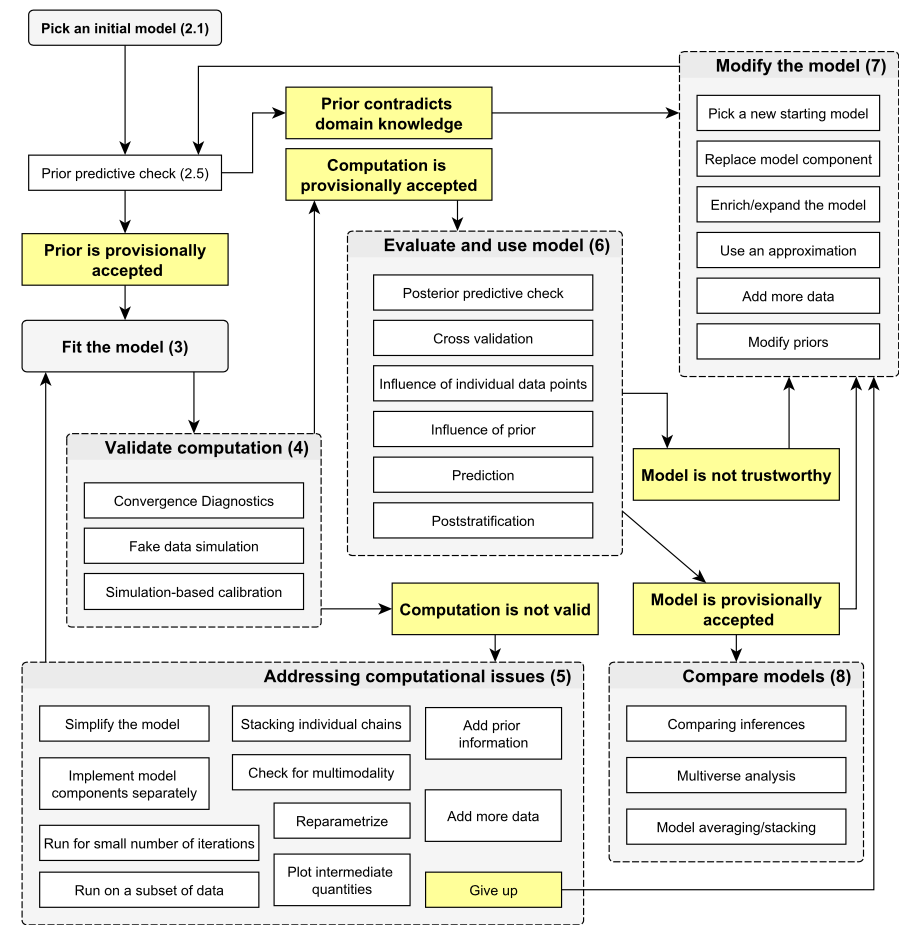
\includegraphics[width=16cm]{./graphics/workflow}
    \label{fig:gelman_wf}
    \caption{Workflow from Gelman et al. (2020).}
\end{figure}


For the sake of completeness, we include a short explanation of each one of the steps in the workflow in Gelman 2020.

\textbf{1. Pick an initial model}

Usually, the starting point is to adapt an idea that already exists in the literature.
This adaptation can be done in different ways: (i) start with a simple model and add layers of complexity, (ii) simplify a complex model, so that it is more understandable or easier to fit while still delivering a similar performance, (iii) consider different starting models with diverging assumptions and follow multiple paths.
Bayesian models are highly modular, as priors and likelihood can be replaced with other distributions if necessary.
Moreover, there is a flexibility regarding how parameter priors interact with each other, which allows for a high degree of model complexity.
Prior predictive checks are a valuable tool when building a model, because it allows to refine the model without without fitting the data multiple times.
This is especially important when the priors should regularize the model to avoid extreme predictions.

Additionally, fully generative model?

In this paper, the initial model is the HB model by \cite{molina_small_2014}.
This model is expanded in (Morelli 2021), where the effect of different likelihoods for income in the logarithmic scale was analyzed with the $t$-distribution providing the best performance over many different scenarios.
The results in these two papers are taken as given and will not be further discussed here.

Multiple models in the appendix? What did not work?

\textbf{2. Fit the model}

Section XY already discussed the two most common Bayesian estimation approaches: MCMC and variational inference.
When fitting a model, the user is confronted with decisions on which algorithm to run and under which conditions.
To make an adequate choice, it is necessary to be aware of the modeling stage.
MCMC provides the most exact approximation, which is more robust with more samples and more chains.
However, if a model was just modified or the user is at an early stage of model development, it is not efficient to fit the model the most exact algorithms and a high number of samples.
Instead, the aim is for the fit of a bad model to fail fast, as models that lead to computational problems are often not adequate.
Such problems can already be clear with just two Markov chain and a drastically lower number of sample than would be taken for final inference.
Even a check with an approximate method such as variational inference might be enough to notice problems with the model, while being drastically faster than HMC.
In this paper, variational algorithms were often used to do a first fit of the model.
While iterating through the models only 2 Markov chains were used and, depending on fitting time, the number of iterations was reduced compared to the degault in \code{Stan}.


\textbf{3. Validate computation}

Diagnostics for Bayesian computation methods were already discussed in Section XY.
In the HMC context, the two main aims are to have no divergences and to have an $\hat R$ lower than 1.01.
All the models presented in this paper fulfill at least these two conditions.
However, adequate diagnostic values are a necessary but not sufficient condition for a reliable model.
To assess model quality, it has to be fitted.
However, using real data can be challenging, as there is no way to distinguish modeling issues from computational issues.
This problem can be avoided by using simulated data, ideally from different scenarios.
Section XY, already presented three scenarios used in this paper.
A model that can fit fake data, is not necessarily correct, but a model that fails when fitting simulating data will also fail with real data.
This paper deals primarily with prediction, so it is enough if samples from the posterior predictive distribution capture the main characteristics of the data.
There will be less emphasis on correcltly recovering parameters from the simulated data.

(Another approach with simulated data is simulation-based calibration.
First, model parameters are generated from the prior and used to simulate data conditional on these values.
Then the model is fitted to data and the posterior is compraed to the simulated parameters from the priors that were used to generate the data.
By repeating this procedure, it is possible to check the inference algorithms – the prior should be recovered when performing inference on data sets drawn from the prior.)

\textbf{4. Address computational issues}

A model that leads to computational problems usually has some underlying modelling issues.
Usually, it is best to start with a simple model and make it more complex one step at a time, making it easier to determine what part of the model is causing problems.
On the other hand, if the model is already complex and shows signs of computational problems, then it is useful to simplify it step by step until the computation is successful.
For example, in a model with numerous groups of random intercepts or random slopes it makes sense to start with just one group and then add each additional group one step at a time, so as to know whether the estimation is working.
A common source of computational problems is prior choice.
Tightening moderately informative priors can help by pushing the sampler towards certain regoins of the parameter space.
However, this adjustment of priors should be in line with available knowledge and not only to solve fitting problems.
One example will be discussed in section XY (prior on shift parameter).

\textbf{5. Evaluate and use the model}

Posterior predictive checks are a useful tool when diagnosing fit problems to the data.
This can be seen as a safeguard against misspecification.
Moreover, such checks might reveal which aspects of the data are not captured well by the model.
Cross-validation is an alternative to posterior predictive checks and has the advantage that part of the data is left out.
Thus, it is less optimistic than posterior predictive checks, which uses the data for model fitting and evaluation.
While refittig model multiple times to do cross-validation can be computationally expensive, there are efficients approximations such as PSIS-LOO.
(Check LOO-PIT in Gabry 2019)

To check how informative the data with respect to a parameter, one can compare the standard deviation of prior and posterior parameters. A higher shrinkage in uncertainty indicates that the data is more informative.

\textbf{6. Modify the model}

Bayesian statistics provides a modular approach in which models can be expanded or reduced in response to new data or failures to fit the model to the data.
Mix of fitting the data and domain expertise.
How are the data linked to the underlying parameters?
How can we use additional data?
The prior is a choice of what kind of available information is integrated into the model and acts as a constraint on the fitting procedure.
There are various levels of priors from completely non-informative to highly informative.
However, the way prior information acts on this information depends on the type of parameter.
Parameters controlling central quantities like a mean are less sensitive to weak prior than scale parameters such as variance.
In turn, scale parameters are less sensitive to weak priors than shape parameters, which control the tails of a distribution.
When expanding the model with additional parameters (e.g., introducing random intercepts or random slopes), it should be considered whether the priors should be tightened to stabilize the estimates, as the amount of data has not changed.

Note that the std. deviation of a $t$-distribution varies with the df.
Joint priors?


\textbf{7. Compare models}

Models are fitted many times, for multiple reasons.
It might be easier to start with simple models, before getting to a more complex model. There are often bugs in the code and in the models.
A model might be well-specified, but it could be improved by expanding it.
The priors might be only placeholders, which will be replaced at a later stage.
Visualize with multiverse comparison.
If many models provide acceptable conclusion, then

Comparing different models is always tied to a certain degree of uncertainty.
Instead of choosing the model with the best cross-validation results, using model stacking can give an insight into model differences.
Stacking combines inferences using a weighting that minimizes cross-validation error (Yao).
Roughly speaking, if a model outperforms another model 80\% of the time, the weights will be 0.8 for the first model and 0.2 for the second model.
This is an indication of model heterogeneity, which can be used as a guide to improve the model.
Thus, stacking is not limited to combine predictions from diferent models.

However, care must be taken when comparing a large number of models to avoid the risk of overfitting.
